\scanpage{40}
\mspage{19}
a) $S'\longrightarrow S^{\deleted{\unsure{'}}}$ surjective, $\widetilde B'\longrightarrow\widetilde A^{\deleted{\unsure{'}}}$ \uline{bijective}

b) \diagram{\begin{tikzcd}
I'\arrow[r,"\sim"]\arrow[d]&I\arrow[d]\\
S'\arrow[r]&S
\end{tikzcd}} commutative

\margin{thus \diagram{\begin{tikzcd}
\widetilde B'\amalg I'\arrow[r,"\sim"]\arrow[d]&\widetilde A\amalg I\arrow[d]\\
S'\arrow[r]&S
\end{tikzcd}} is commutative.}

c) $\forall\alpha\in S$, the subgraph $G'(\alpha)$ of $G'$ [formed by the \deleted{\unsure{$S$}} $s'\in S'$ over $\alpha$, and the \deleted{arrows} arcs $a'\in\widetilde A'$ which are in $\inserted{\widetilde C'=}\widetilde A'\setminus\widetilde B'$ (i.e. over $\operatorname{id}_\alpha$) and whose origin (thus the endpoint too) is in $S'_\alpha$], equipped with \deleted{\unsure{and by} $\unsure{\widetilde A_\alpha|\widetilde A}$ \unsure{or|and} $\unsure{A}$} $I'_\alpha\inserted{\amalg\widetilde B'_\alpha}\longrightarrow S'_\alpha$ induced by $\inserted{\widetilde B'\amalg}I'\unsure{\to|{-}}S'$, and with $\gamma_\alpha:S'_\alpha\longrightarrow\mathbb N$ induced by $\unsure{g'|f'}:S'\unsure{\to|{-}}\mathbb N$, is an \uline{MD-graph} \inserted{$\underline G'(\alpha)$} \deleted{\unsure{of type|of genus} $\unsure{g=g(\alpha)|(g_\alpha,\nu_\alpha)}$\unsure{, i.e.}}, i.e. it is \uline{connected}, \deleted{[NB it \unsure{automatically satisfies}} \inserted{and [it satisfies all}\deleted{\unsure{the}} \inserted{the} rigidity conditions relative to the vertices $\beta$ such that, \deleted{\unsure{$\alpha$}} $g'_\beta\in\{0,1\}$, namely that

\margin{\uline{NB} $\widetilde B'_\alpha$ is the set of $\vec a'\in\widetilde B'_\alpha$ whose origin lies in $S'_\alpha$, i.e. in $G'(\alpha)$, thus $\widetilde B'_\alpha\xrightarrow{\sim}\widetilde A_\alpha$}

\figure{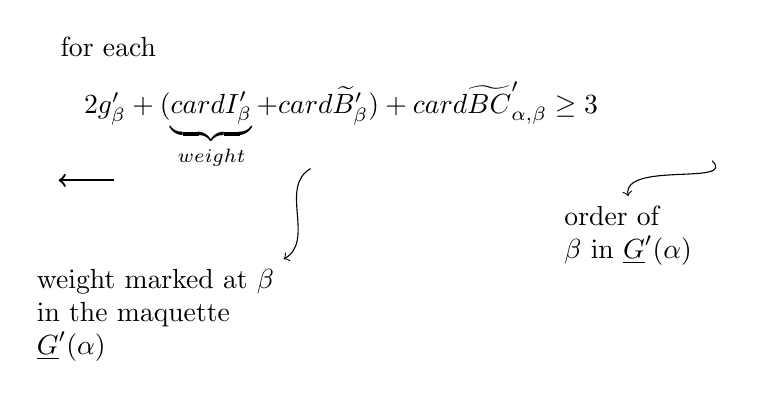
\begin{tikzpicture}[x=1cm,y=1cm]
\node[anchor=west] (eq) at (0,0) {$2g'_\beta+(\underbrace{\operatorname{card}I'_\beta}_{\deleted{\unsure{weight}}}\inserted{+\operatorname{card}\widetilde B'_\beta)}+\operatorname{card}\widetilde{\deleted{B}\inserted{C}}'_{\deleted{\unsure{\alpha}},\beta}\geq3$};
\node[anchor=north west,align=left] (mark) at (-0.6,-1.7) {weight marked at $\beta$\\in the maquette\\$\underline G'(\alpha)$};
\node[anchor=north west,align=left] (ord) at (6.1,-0.9) {order of\\$\beta$ in $\underline G'(\alpha)$};
\draw[->,thick] (0.5,-0.7)--(-0.2,-0.7);
\draw[->] (3.0,-0.55) to[out=210,in=30] (mark.north east);
\draw[->] (8.1,-0.45) to[out=-45,in=100] (ord.north);
\node[anchor=west] at (-0.3,1.0) {\deleted{\unsure{for each}}};
\end{tikzpicture}}

\margin{for the condition is \unsure{automatically ensured} \deleted{\unsure{a priori} $\unsure{2g'_\beta}$ \unsure{is}} \deleted{\unsure{since it is}} \unsure{equivalent to} : \figure{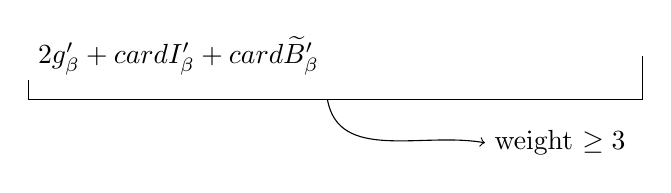
\begin{tikzpicture}[x=1cm,y=1cm]
\node[anchor=west] at (0,0) {$2g'_\beta+\operatorname{card}I'_\beta+\operatorname{card}\widetilde B'_\beta$};
\draw (0,-0.3)--(0,-0.55)--(7.8,-0.55)--(7.8,0);
\draw[->] (3.8,-0.55) to[out=-80,in=170] (5.8,-1.1);
\node[anchor=west] at (5.8,-1.1) {weight $\geq3$};
\end{tikzpicture}}}

\margin{\unsure{\deleted{$\operatorname{card}I_\beta$}}}

\deleted{\unsure{which a priori} \unsure{$+\operatorname{car}$} $\left[2g'_\beta+\operatorname{card}I'_\beta\geq3\right]$ $2g'_\beta+\operatorname{card}I'_\beta+\operatorname{card}\widetilde A'_\beta\geq3)$ which a priori is a weaker condition (since $\underline G'$ is an MD-graph)\ldots}

d) the genus of the MD-graph $\underline G(\alpha)$ is equal to $g_\alpha$, i.e. we have
\[
\sum_{\beta\in S'_\alpha}g'_\beta+h_1(G(\alpha))=g_\alpha.
\]
\mspage{39}
